% $Header: /cvsroot/latex-beamer/latex-beamer/solutions/conference-talks/conference-ornate-20min.en.tex,v 1.6 2004/10/07 20:53:08 tantau Exp $

\documentclass{beamer}

% This file is a solution template for:

% - Talk at a conference/colloquium.
% - Talk length is about 20min.
% - Style is ornate.



% Copyright 2004 by Till Tantau <tantau@users.sourceforge.net>.
%
% In principle, this file can be redistributed and/or modified under
% the terms of the GNU Public License, version 2.
%
% However, this file is supposed to be a template to be modified
% for your own needs. For this reason, if you use this file as a
% template and not specifically distribute it as part of a another
% package/program, I grant the extra permission to freely copy and
% modify this file as you see fit and even to delete this copyright
% notice.


\mode<presentation>
{
%  \usetheme{Warsaw}
%  \usetheme{Boadilla}
%  \usetheme{Goettingen}
%  \usetheme{Hannover}
%  \usetheme{Madrid}
%  \usetheme{Marburg}
%  \usetheme{Montpellier}
%  \usetheme{Pittsburgh}
  \usetheme{Hawke}
  % or ...

  \setbeamercovered{transparent}
  % or whatever (possibly just delete it)
}


\usepackage[english]{babel}
% or whatever

\usepackage[latin1]{inputenc}
% or whatever

\usepackage{times}
\usepackage[T1]{fontenc}
% Or whatever. Note that the encoding and the font should match. If T1
% does not look nice, try deleting the line with the fontenc.

\usepackage{multimedia}


%%%%%%
% My Commands
%%%%%%

\newcommand{\ml}{{\sc matlab}}

%%%%

\title[Lecture 8] % (optional, use only with long paper titles)
{Lecture 8 - Example iteration methods and speed}

% \subtitle
% {Include Only If Paper Has a Subtitle}

\author[I. Hawke] % (optional, use only with lots of authors)
{I.~Hawke}
% - Give the names in the same order as the appear in the paper.
% - Use the \inst{?} command only if the authors have different
%   affiliation.

\institute[University of Southampton] % (optional, but mostly needed)
{
%  \inst{1}%
  School of Mathematics, \\
  University of Southampton, UK
}
% - Use the \inst command only if there are several affiliations.
% - Keep it simple, no one is interested in your street address.

\date[Semester 1] % (optional, should be abbreviation of conference name)
{MATH3018/6141, Semester 1}
% - Either use conference name or its abbreviation.
% - Not really informative to the audience, more for people (including
%   yourself) who are reading the slides online

\subject{Numerical methods}
% This is only inserted into the PDF information catalog. Can be left
% out.



% If you have a file called "university-logo-filename.xxx", where xxx
% is a graphic format that can be processed by latex or pdflatex,
% resp., then you can add a logo as follows:

\pgfdeclareimage[height=0.5cm]{university-logo}{mathematics_7469}
\logo{\pgfuseimage{university-logo}}



% Delete this, if you do not want the table of contents to pop up at
% the beginning of each subsection:
%  \AtBeginSubsection[]
%  {
%    \begin{frame}<beamer>
%      \frametitle{Outline}
%      \tableofcontents[currentsection,currentsubsection]
%    \end{frame}
%  }
\AtBeginSection[]
{
  \begin{frame}<beamer>
    \frametitle{Outline}
    \tableofcontents[currentsection]
  \end{frame}
}


% If you wish to uncover everything in a step-wise fashion, uncomment
% the following command:

%\beamerdefaultoverlayspecification{<+->}


\begin{document}

\begin{frame}
  \titlepage
\end{frame}


\section{Speed of convergence}

\subsection{Speed of convergence}

\begin{frame}
  \frametitle{Brief reminders}

  Previously: finding root of $f$, i.e.\ solution to
  \begin{equation*}
    f(x) = 0.
  \end{equation*}
  Iteration: define sequence $\{x_n\}$ using map $g : x_n
  \rightarrow x_{n+1}$. Map designed such that fixed points of
  $g$ are roots of $f$. If sequence converges, have found a root. \pause

  \vspace{1ex}

  For a contraction mapping with Lipschitz constant $L < 1$ map converges, with error
  \begin{equation*}
    |e_n| \leq \frac{L^n}{1 - L} |x_1 - x_0|.
  \end{equation*} \pause

  \vspace{1ex}

  Error depends on worst case value of $L$ in whole interval. Often find faster convergence for better initial guesses.

\end{frame}

\begin{frame}
  \frametitle{Speed of convergence}

  \begin{overlayarea}{\textwidth}{0.9\textheight}
    \only<1-|handout:1->
    {
      Expect speed of convergence to depend on map $g$ near root $s$. Can show this for ``nice'' $g$ and ``good'' $x_n$.
    }
    \only<2-|handout:1->
    {
      Define error at $n^{\text{th}}$ stage
      \begin{equation*}
        e_n = x_n - s.
      \end{equation*}
      As $s$ is a fixed point of $g$, use Taylor expansion of $e_{n+1}$:
      \begin{align*}
        e_{n+1} = x_{n+1} - s & = g(x_n) - g(s) \\
        & = g'(s) (x_n - s) + \tfrac{1}{2!} g''(s) (x_n - s)^2 + \dots \\
        & = g'(s) e_n + \tfrac{1}{2!} g''(s) e_n^2 + \dots
      \end{align*}
    }
    \only<3|handout:1>
    {
      If error small then a \emph{linear} or \emph{first order} method converges as
      \begin{equation*}
        e_{n+1} \sim g'(s) e_n;
      \end{equation*}
      decreases by a constant amount each step, proportional to the derivative of the map at the root.
    }
    \only<4-|handout:2>
    {
      If $g'(s) \equiv 0$ and error small a \emph{quadratic} or \emph{second
        order} map converges as
      \begin{equation*}
        e_{n+1} \sim g''(s) e_n^2.
      \end{equation*}
    }
    \only<5-|handout:2>
    {

      The more derivatives of $g$ that vanish at the root, the faster
      the convergence (but the better the guess must be).
    }
  \end{overlayarea}

\end{frame}


\section{Example methods}


\subsection{General framework}

\begin{frame}
  \frametitle{General framework}

  As usual we are trying to solve
  \begin{equation*}
    f(x) = 0
  \end{equation*}
  for $x \in [a,b]$. Functional iteration is map
  \begin{equation*}
    g(x) = x - f(x);
  \end{equation*}
  at fixed points of this map $f(x)$ must vanish. \pause

  \vspace{1ex}

  Simple generalization: introduce $\varphi(x) \neq 0$, then
  \begin{equation*}
    g(x) = x - \varphi(x) f(x)
  \end{equation*}
  also has that $g(s) = s \, \implies \, f(s) = 0 \, \implies$ root. \pause

  \vspace{1ex}

  Increase speed of convergence by choice of $\varphi$, provided
  \begin{equation*}
    0 < \varphi(x) < \infty, \quad x \in [a, b].
  \end{equation*}

\end{frame}


\subsection{Chord method}

\begin{frame}
  \frametitle{Chord method}

  Simplest choice: $\varphi(x) = m \neq 0$, giving
  \begin{equation*}
    g(x) = x - m f(x).
  \end{equation*}
  This is known as the \emph{chord method}. \pause

  \vspace{1ex}

  Free to choose $m$, provided that $g$ is a contraction
  mapping in $[a,b]$. Requires $|g'(x)| < 1$ in interval; implies
  \begin{align*}
    && | 1 - m f'(x) | & < 1 & \forall x & \in [a,b] \\
    \Rightarrow && 0 < m f'(x) & < 2 & \forall x & \in [a,b].
  \end{align*} \pause

  If $m = 1 / f'(s)$ then method converges quadratically.

\end{frame}

\begin{frame}
  \frametitle{Chord method: geometric picture}

  \begin{columns}
    \begin{column}{0.5\textwidth}

      Usual geometric picture: move on horizontal and vertical lines from map to $y=x$ and axis.

      \vspace{2ex}

      Chord method geometric picture: move on lines of constant slope
      $1/m$ from map to axis to find next $x_n$.

      \vspace{2ex}

      Note that this plot uses $f(x)$; the previous plots used $g(x)$.
    \end{column}
    \begin{column}{0.5\textwidth}
      \begin{center}
        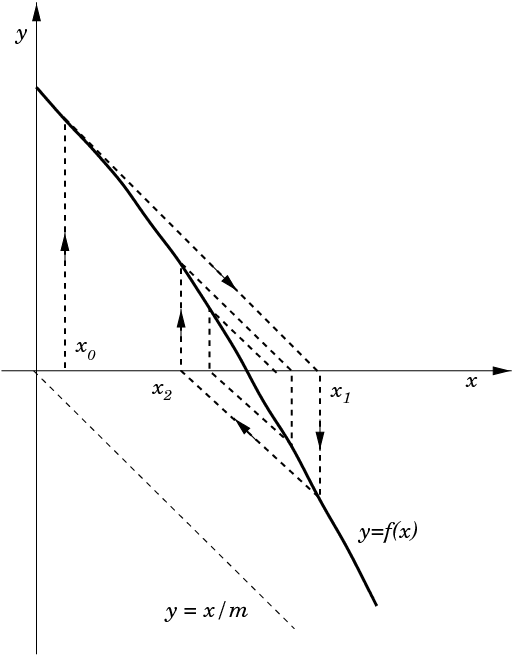
\includegraphics[width=\textwidth]{figures/chord}
      \end{center}
    \end{column}
  \end{columns}

\end{frame}

\begin{frame}
  \frametitle{Example of the chord method}

  We look at
  \begin{equation*}
    f(x) = x - \cos(x), \quad x \in [0, 1].
  \end{equation*}\pause
  The generic chord method has map
  \begin{equation*}
    g(x) = x ( 1 - m ) + m \cos(x),
  \end{equation*}
  and the range of allowable $m$ values is
  \begin{equation*}
    0 <  | m + m \sin(x) | < 2
  \end{equation*}
  implying $0<|m|<2$ and $0<|1.8415 m|<2$. \pause Choosing $m = 1.08 \,
  (\lesssim 2 / 1.8415)$ we obtain the iteration map
  \begin{equation*}
    x_{n+1} = -0.08 x_n + 1.08 \cos(x_n).
  \end{equation*}

\end{frame}

\begin{frame}
  \frametitle{Example of the chord method - 2}

  \begin{columns}
    \begin{column}{0.5\textwidth}
      \begin{overlayarea}{\textwidth}{0.9\textheight}
        \only<1-|handout:1->
        {
          Sequence produced by map
          \begin{equation*}
            x_{n+1} = -0.08 x_n + 1.08 \cos(x_n)
          \end{equation*}
          starting from zero is
          \begin{align*}
            x_0 & = 0 \\
            x_1 & =    1.0800 \\
            x_2 & =    0.4226 \\
            x_3 & =    0.9512 \\
            x_4 & =    0.5511 \\
            x_5 & = 0.8760
          \end{align*}
        }
        \only<5|handout:2>
        {
          converges linearly to solution $s = 0.739085\dots$.
        }
      \end{overlayarea}
    \end{column}
    \begin{column}{0.5\textwidth}
      \begin{overlayarea}{\textwidth}{0.6\textheight}
        \only<1|handout:0>
        {
          \begin{center}
            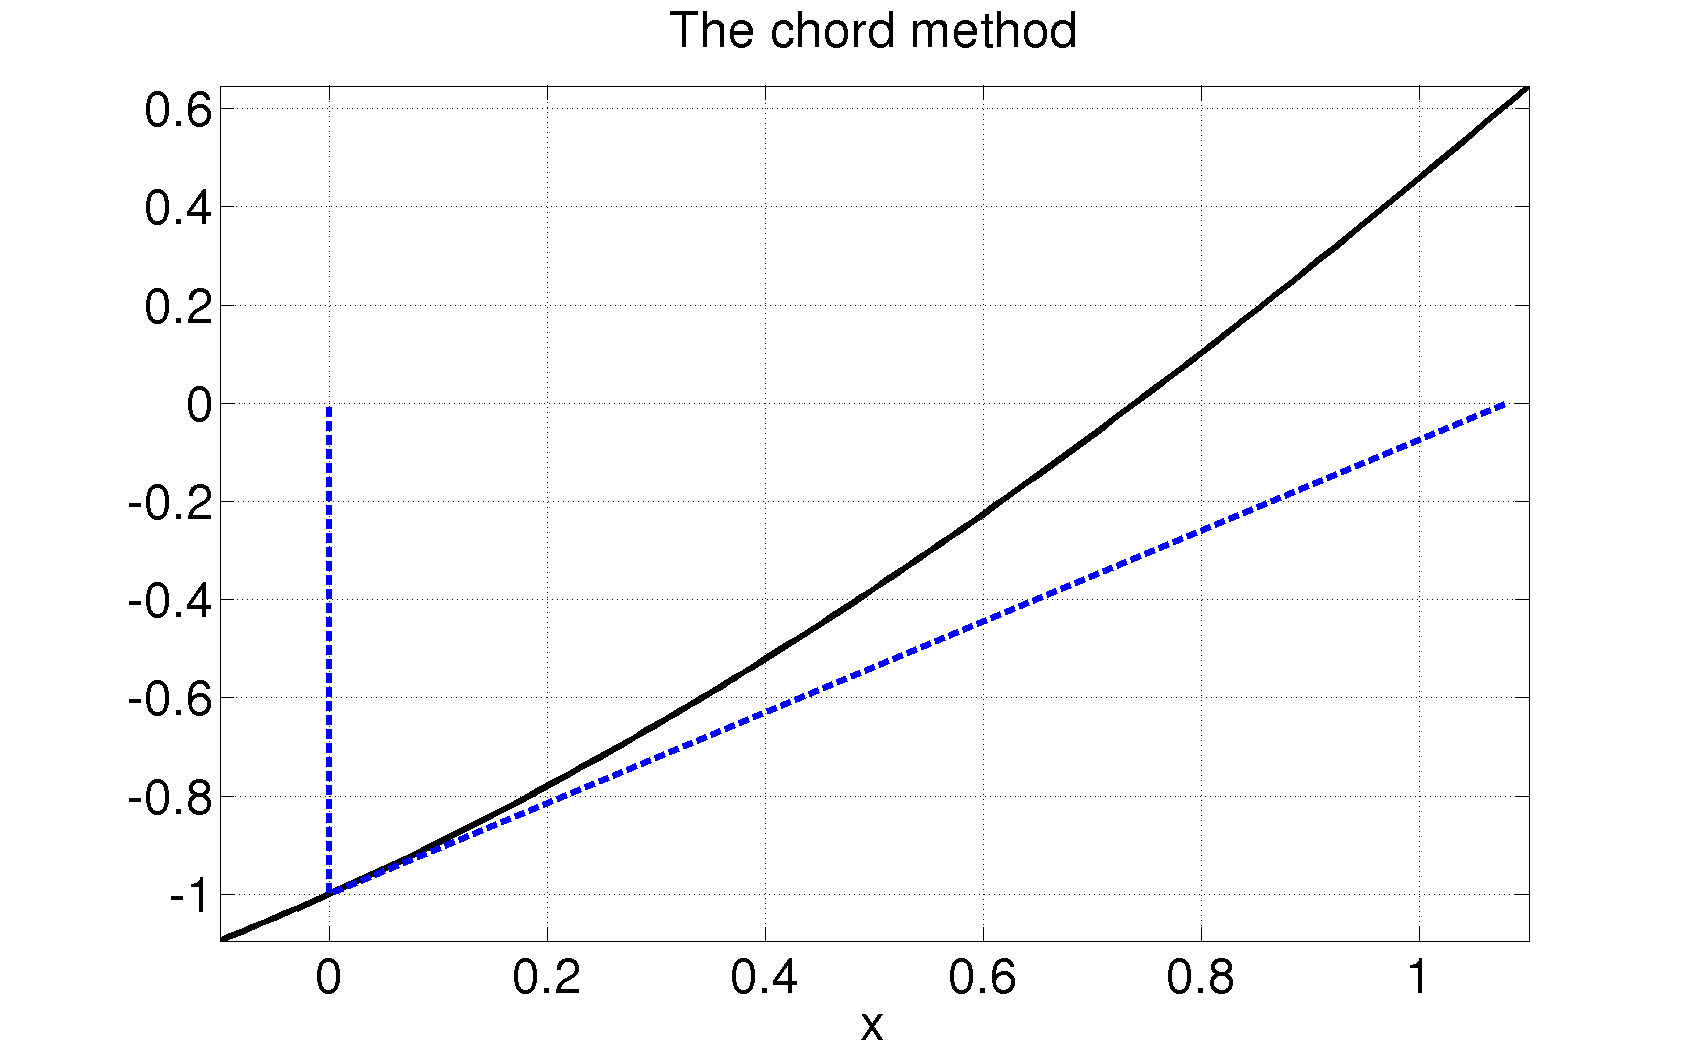
\includegraphics[width=\textwidth]{figures/ChordMap2}
          \end{center}
        }
        \only<2|handout:0>
        {
          \begin{center}
            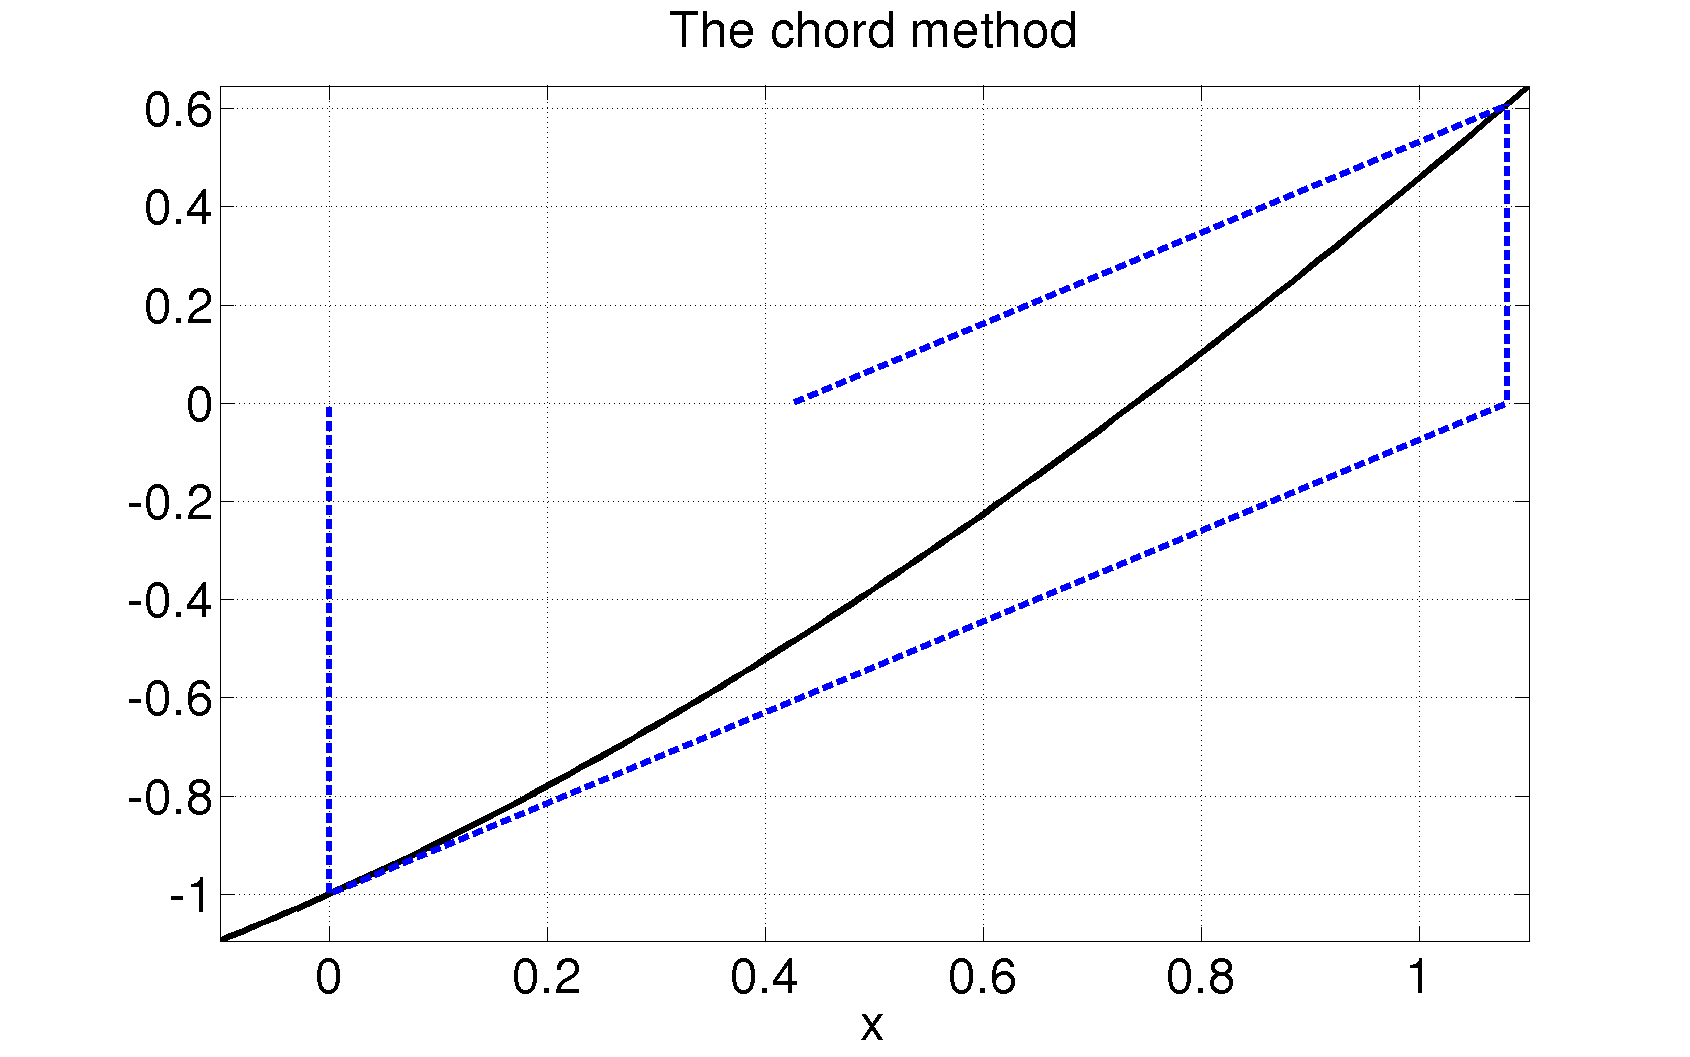
\includegraphics[width=\textwidth]{figures/ChordMap3}
          \end{center}
        }
        \only<3|handout:0>
        {
          \begin{center}
            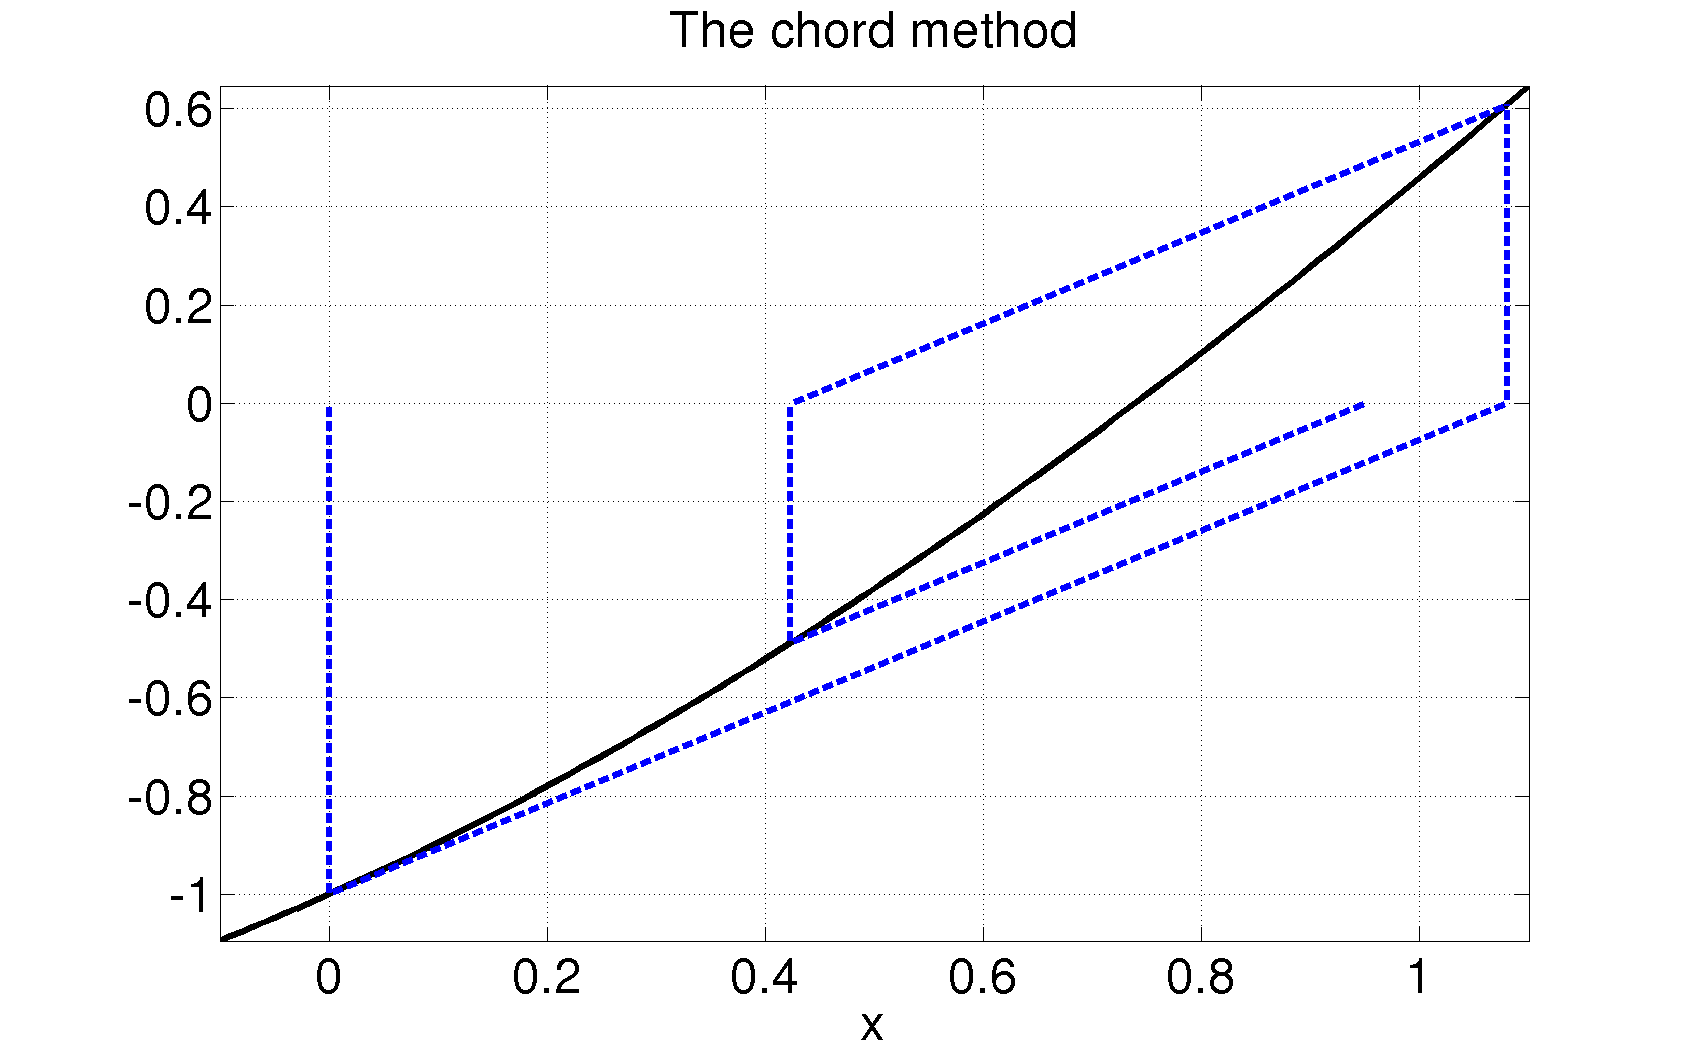
\includegraphics[width=\textwidth]{figures/ChordMap4}
          \end{center}
        }
        \only<4|handout:1>
        {
          \begin{center}
            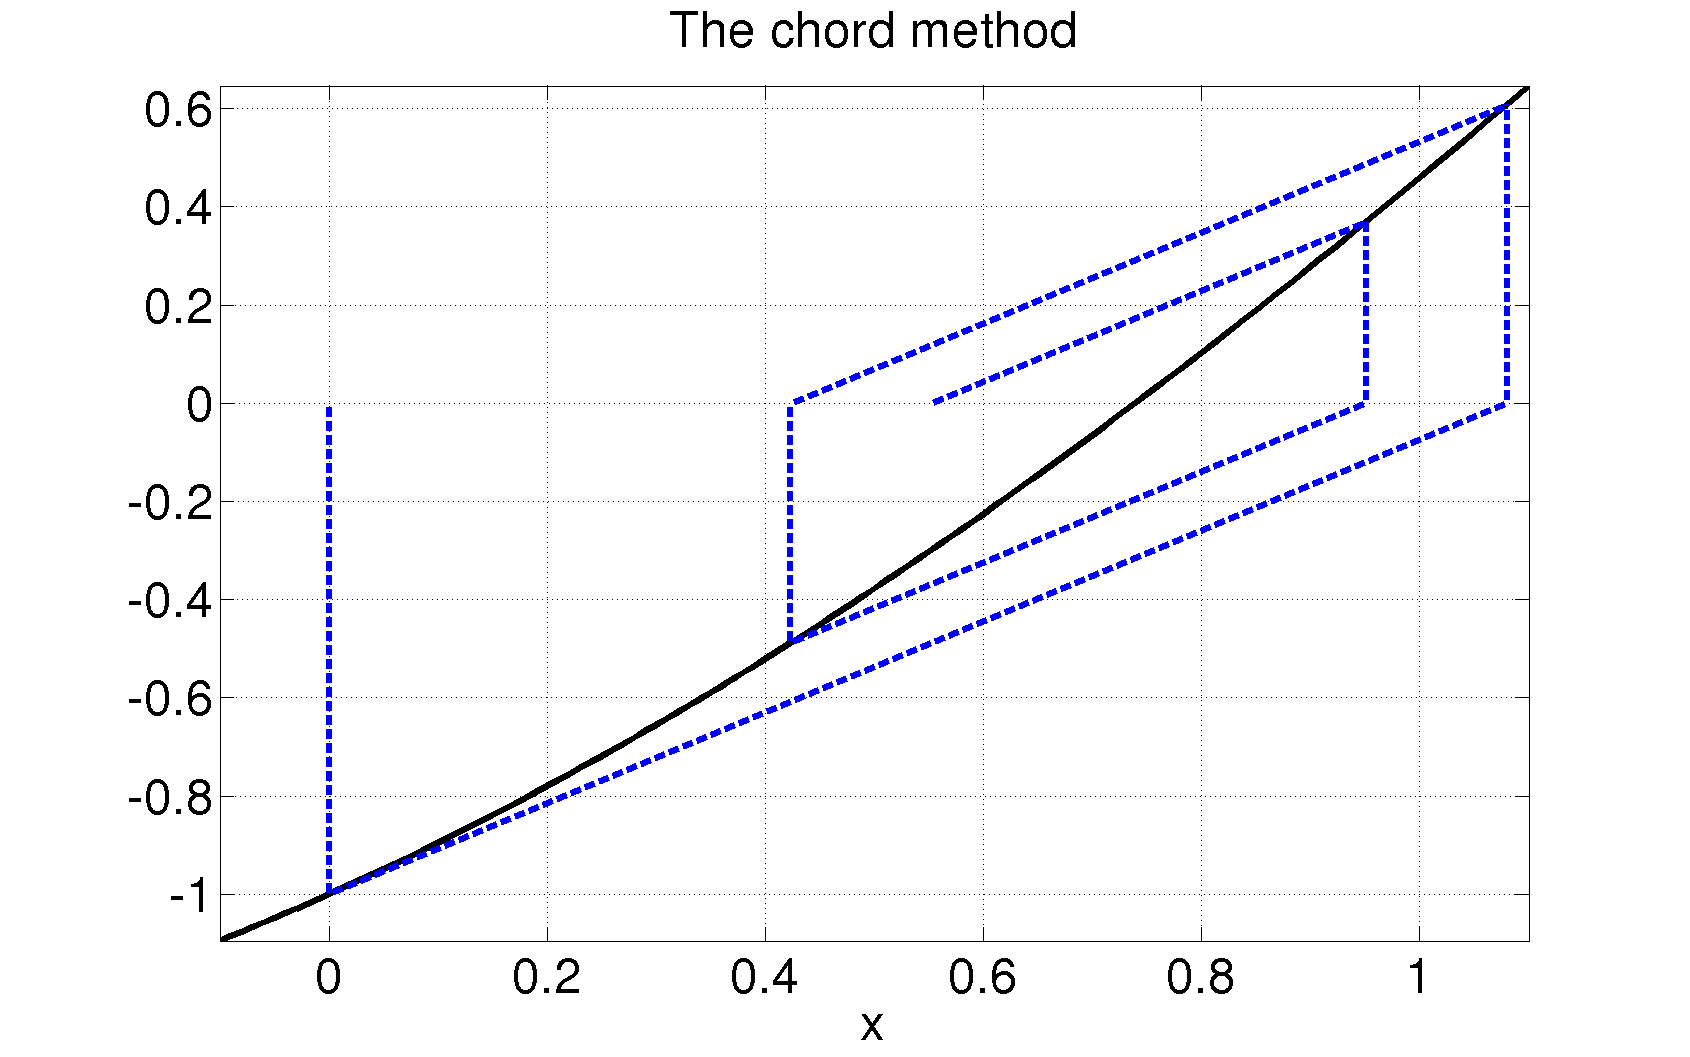
\includegraphics[width=\textwidth]{figures/ChordMap5}
          \end{center}
        }
        \only<5|handout:2>
        {
          \begin{center}
            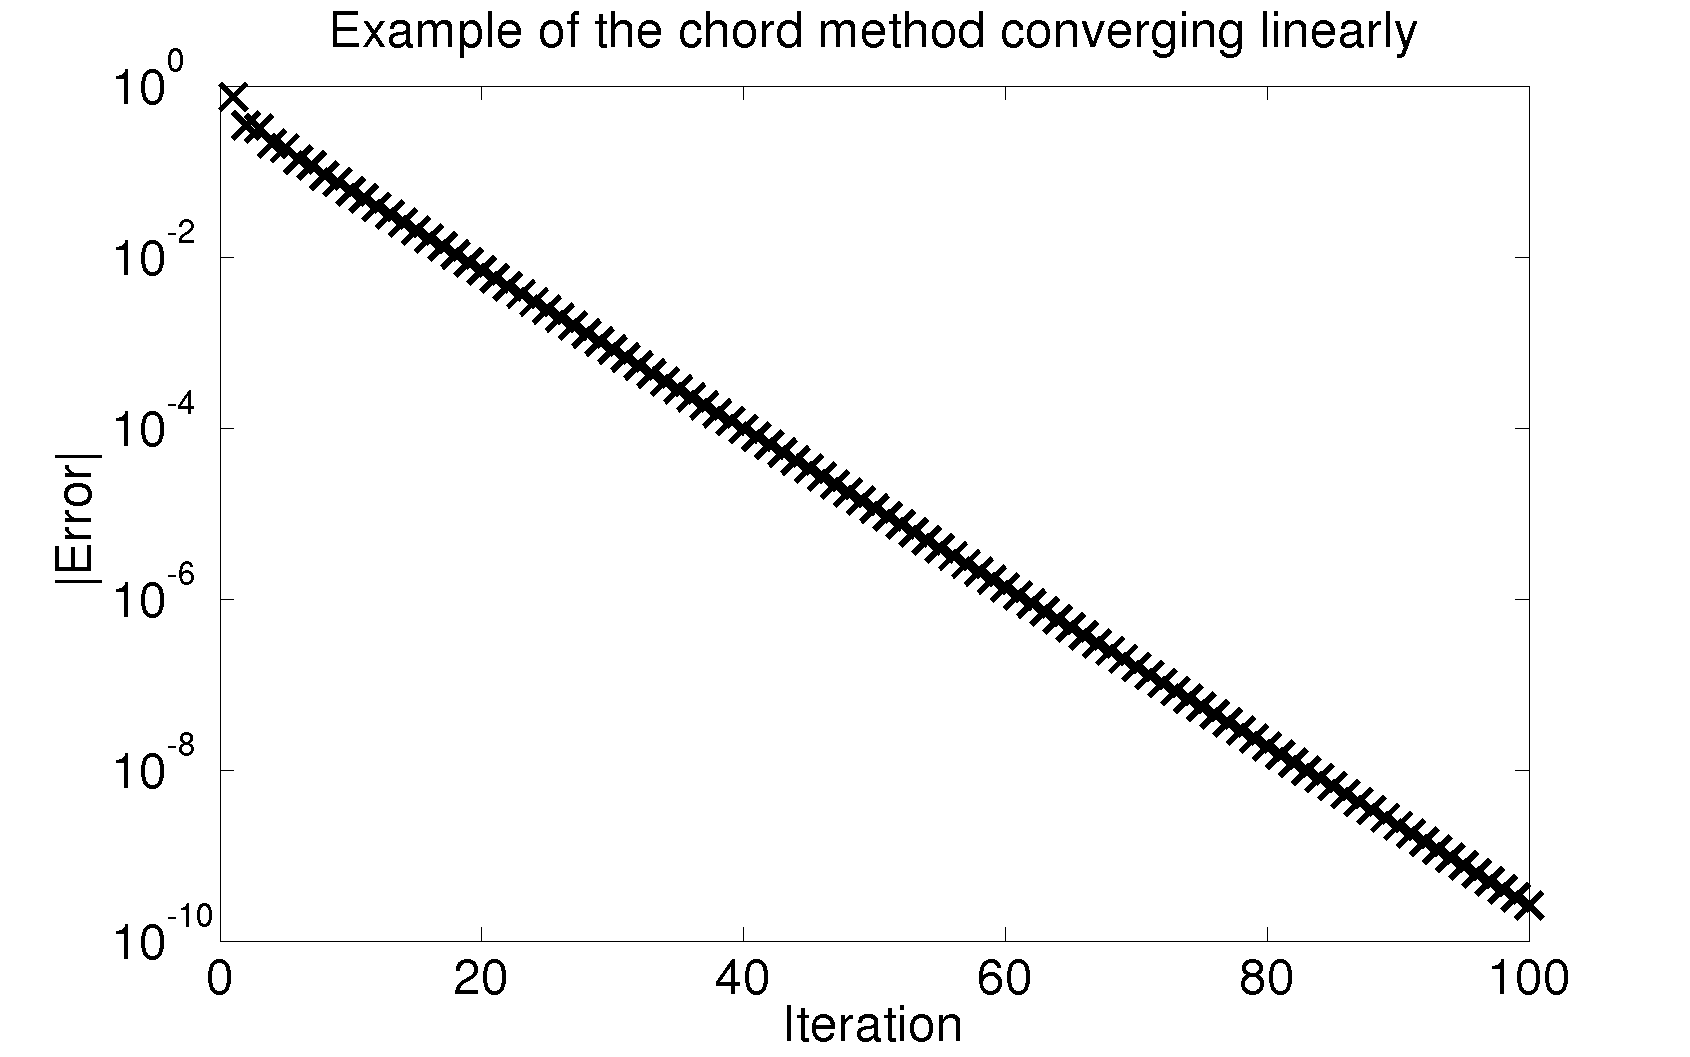
\includegraphics[width=\textwidth]{figures/Chord1}
          \end{center}
        }
      \end{overlayarea}
    \end{column}
  \end{columns}
\end{frame}


\subsection{Newton's method}

\begin{frame}
  \frametitle{Newton's method}

  For quadratic convergence need $g'(s) \equiv 0$. Newton's method: choose
  %
  \begin{equation*}
    \varphi(x)  = \frac{1}{f'(x)} \quad \implies \quad g(x)  = x - \frac{f(x)}{f'(x)}.
  \end{equation*} \pause
  %
  A simple check shows
  \begin{equation*}
    g'(s)  = 1 - 1 + \frac{f(s) f''(s)}{\left( f'(s) \right)^2} = 0.
  \end{equation*} \pause
  %
  The iteration scheme is
  \begin{equation*}
    x_{n+1} = x_n - \frac{f(x_n)}{f'(x_n)};
  \end{equation*}
  more complex, has limitations: \pause
  %
  \begin{itemize}
  \item Needs derivative. If unknown, better to use secant method.
  \item If derivative vanishes at root, speed of convergence calculation is wrong. Problem for multiple roots, for which Newton's method converges at best linearly.
  \end{itemize}

\end{frame}

\begin{frame}
  \frametitle{Newton's method: geometric picture}

  \begin{columns}
    \begin{column}{0.5\textwidth}
      Geometric picture for Newton's method: move on lines
      with slope given by derivative at $x_n$.
    \end{column}
    \begin{column}{0.5\textwidth}
      \begin{center}
        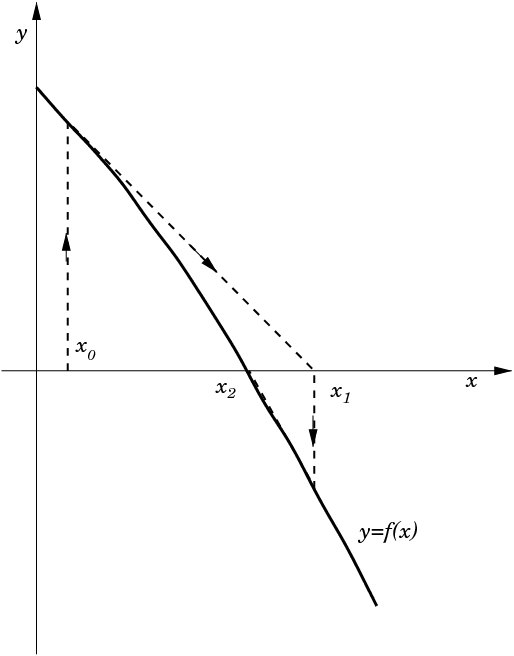
\includegraphics[width=\textwidth]{figures/Newton}
      \end{center}
    \end{column}
  \end{columns}

\end{frame}

\begin{frame}
  \frametitle{Example of Newton's method}

  We again look at
  \begin{equation*}
    f(x) = x - \cos(x), \quad x \in [0, 1].
  \end{equation*}
  Newton's method has map
  \begin{align*}
    g(x) & = x - \frac{f(x)}{f'(x)} \\
    & = \frac{x \sin(x) + \cos(x)}{1 + \sin(x)}.
  \end{align*}
  As $f' \ne 0$ in the domain, expect quadratic convergence.

\end{frame}

\begin{frame}
  \frametitle{Example of Newton's method - 2}

  \begin{columns}
    \begin{column}{0.5\textwidth}
      \begin{overlayarea}{\textwidth}{0.9\textheight}
        \only<1-|handout:1->
        {
          Sequence produced by map
          \begin{equation*}
            x_{n+1} = \frac{x_n \sin(x_n) + \cos(x_n)}{1 + \sin(x_n)},
          \end{equation*}
          starting from zero is
          \begin{align*}
            x_0 & = 0.0000000000 \\
            x_1 & = 1.0000000000 \\
            x_2 & = 0.7503638678 \\
            x_3 & = 0.7391128909 \\
            x_4 & = 0.7390851334 \\
            x_5 & = 0.7390851332
          \end{align*}
        }
        \only<3|handout:2>
        {
          converges quadratically to solution $s =
          0.739085\dots$.
        }
      \end{overlayarea}
    \end{column}
    \begin{column}{0.5\textwidth}
      \begin{overlayarea}{\textwidth}{0.6\textheight}
        \only<1|handout:0>
        {
          \begin{center}
            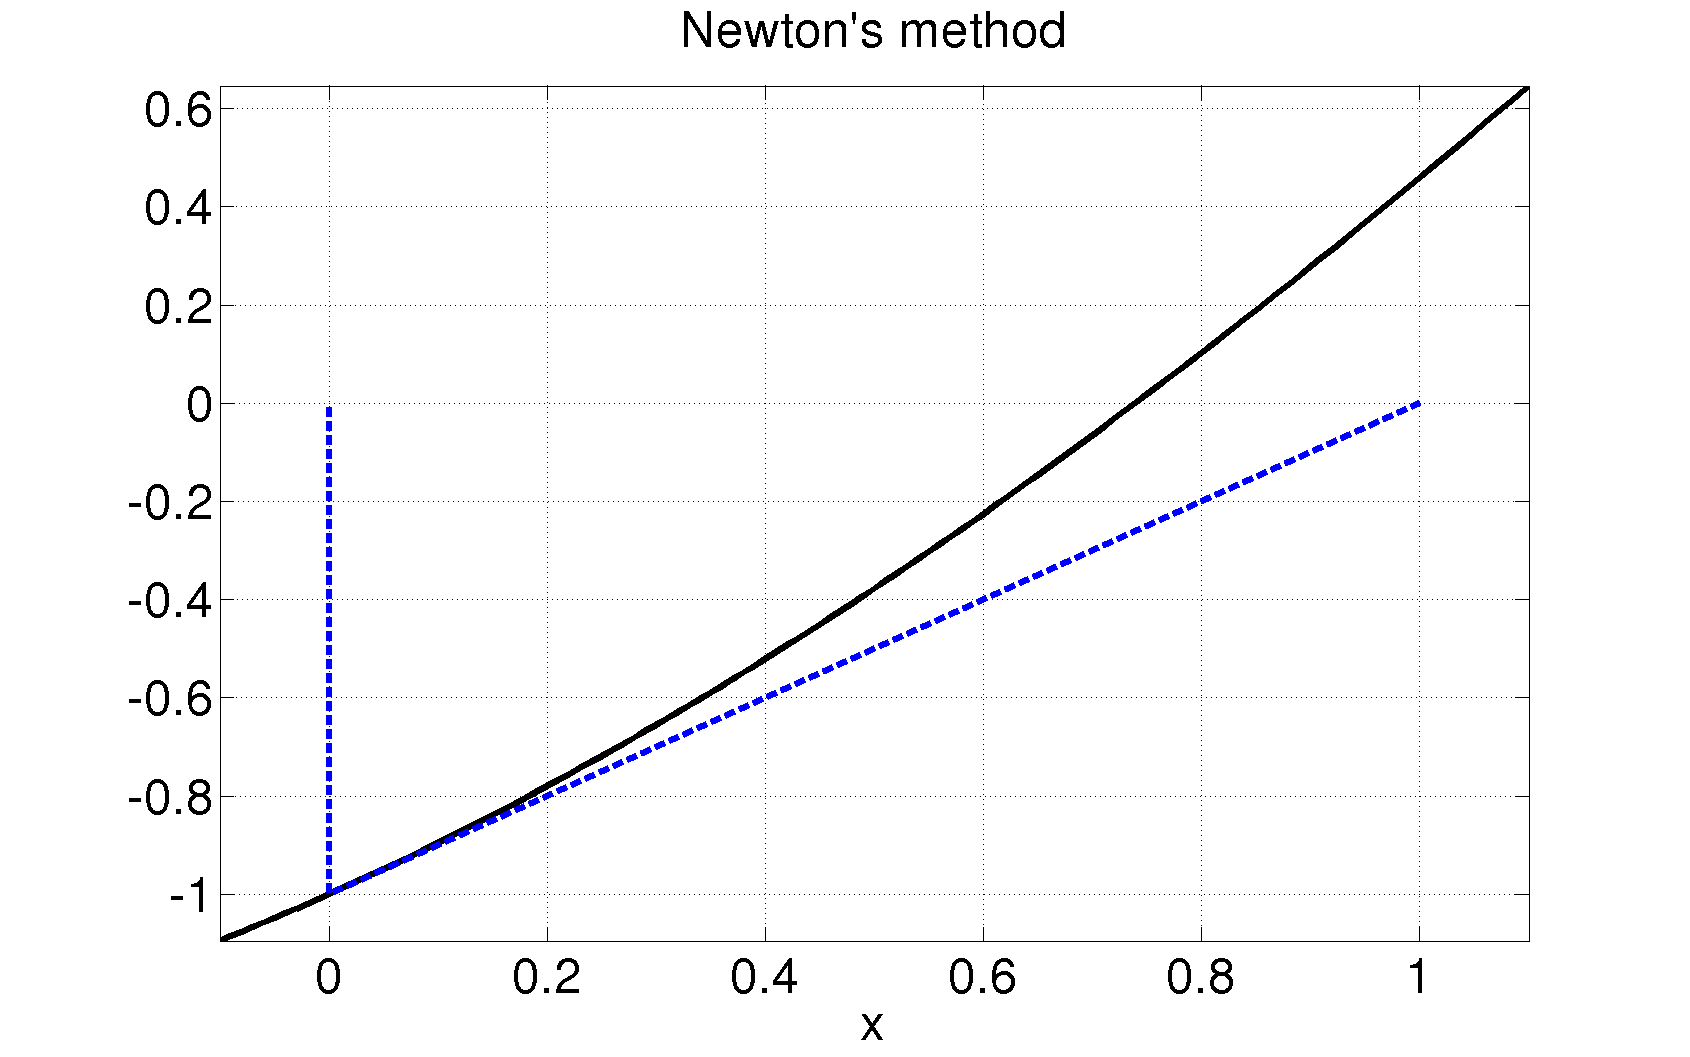
\includegraphics[width=\textwidth]{figures/NewtonMap2}
          \end{center}
        }
        \only<2|handout:1>
        {
          \begin{center}
            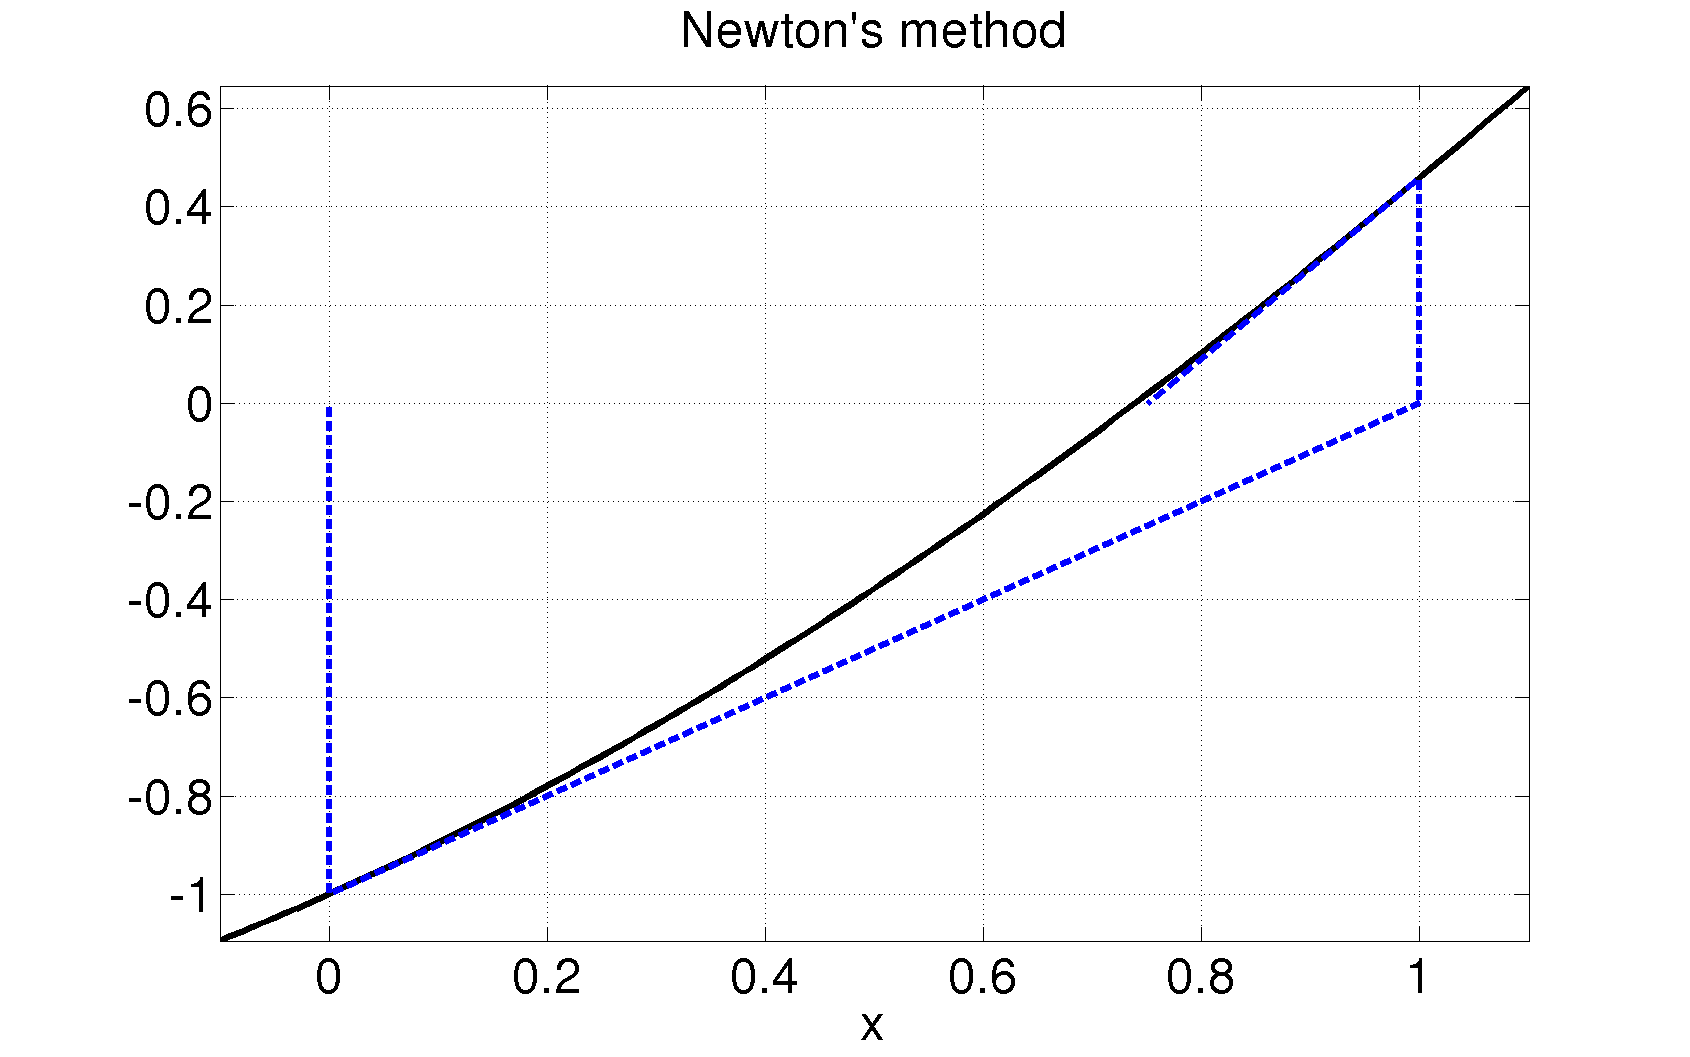
\includegraphics[width=\textwidth]{figures/NewtonMap3}
          \end{center}
        }
        \only<3|handout:2>
        {
          \begin{center}
            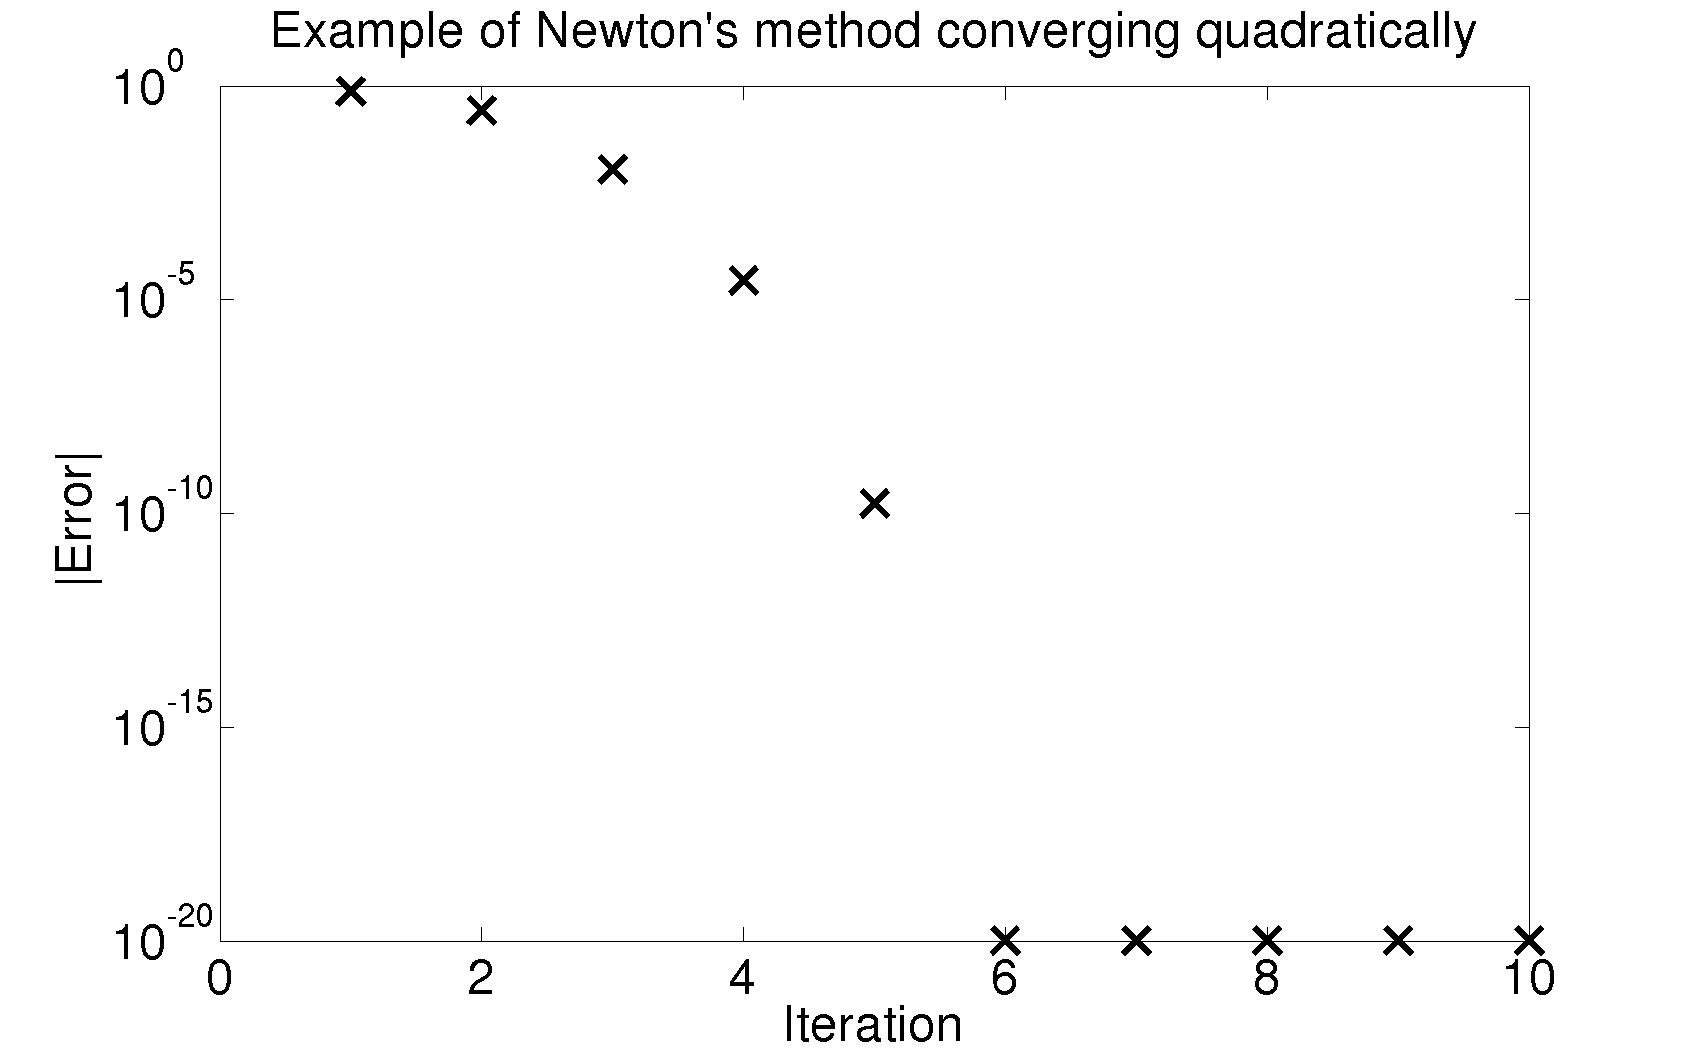
\includegraphics[width=\textwidth]{figures/Newton1}
          \end{center}
        }
      \end{overlayarea}
    \end{column}
  \end{columns}
\end{frame}


\subsection{Secant method}

\begin{frame}
  \frametitle{Secant method}

  Key disadvantage of Newton's method: needs derivative $f'(x)$. Extra function evaluations add cost, even where derivative can be computed. The Secant Method instead approximates derivative using
  \begin{equation*}
    f'(x_n) \simeq \frac{f \left (x_n \right ) - f \left ( x_{n-1}
      \right )}{x_n - x_{n-1}} .
  \end{equation*}
  This results in the iteration scheme
  \begin{equation*}
    x_{n+1} = x_n - f(x_n) \frac{x_n - x_{n-1}}{f(x_n) - f(x_{n-1})}.
  \end{equation*} \pause

  Does not match framework: \emph{two} previous values in sequence. Means two initial guesses required, and contraction mapping theorems cannot be used.  Can show that method converges; often more useful and faster than Newton's method.

\end{frame}


\begin{frame}
  \frametitle{Secant method: geometric picture}

  \begin{columns}
    \begin{column}{0.5\textwidth}
      Geometric picture for Secant method: move on lines whose slope is determined by secant to function through $x_{n-1}, x_n$.
    \end{column}
    \begin{column}{0.5\textwidth}
      \begin{center}
        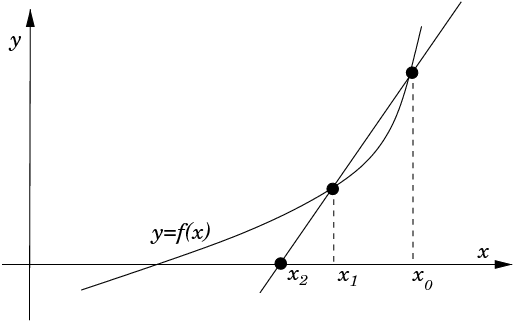
\includegraphics[width=\textwidth]{figures/secant}
      \end{center}
    \end{column}
  \end{columns}

\end{frame}

\begin{frame}
  \frametitle{Example of the Secant method}

  Again look at
  \begin{equation*}
    f(x) = x - \cos(x), \quad x \in [0, 1].
  \end{equation*}
  The Secant method has the iteration scheme (no map!)
  \begin{equation*}
    x_{n+1}  = x_n - f(x_n) \frac{x_n - x_{n-1}}{f(x_n) - f(x_{n-1})}.
  \end{equation*}
  Expect slightly slower convergence than Newton's method.

\end{frame}

\begin{frame}
  \frametitle{Example of the Secant method - 2}

  \begin{columns}
    \begin{column}{0.5\textwidth}
      \begin{overlayarea}{\textwidth}{0.9\textheight}
        \only<1-|handout:1->
        {
          Sequence uses iteration
          \begin{equation*}
            x_{n+1} = x_n - f(x_n) \frac{x_n - x_{n-1}}{f(x_n) - f(x_{n-1})},
          \end{equation*}
          starting from $x_0=0,x_1=1$:
          \begin{align*}
            x_0 & = 0.0000000000 \\
            x_1 & = 1.0000000000 \\
            x_2 & = 0.6850733573 \\
            x_3 & = 0.7362989976 \\
            x_4 & = 0.7391193619 \\
            x_5 & = 0.7390851121
          \end{align*}
        }
        \only<3|handout:2>
        {
          converges to solution $s = 0.739085\dots$.
        }
      \end{overlayarea}
    \end{column}
    \begin{column}{0.5\textwidth}
      \begin{overlayarea}{\textwidth}{0.9\textwidth}
        \only<1|handout:0>
        {
          \begin{center}
            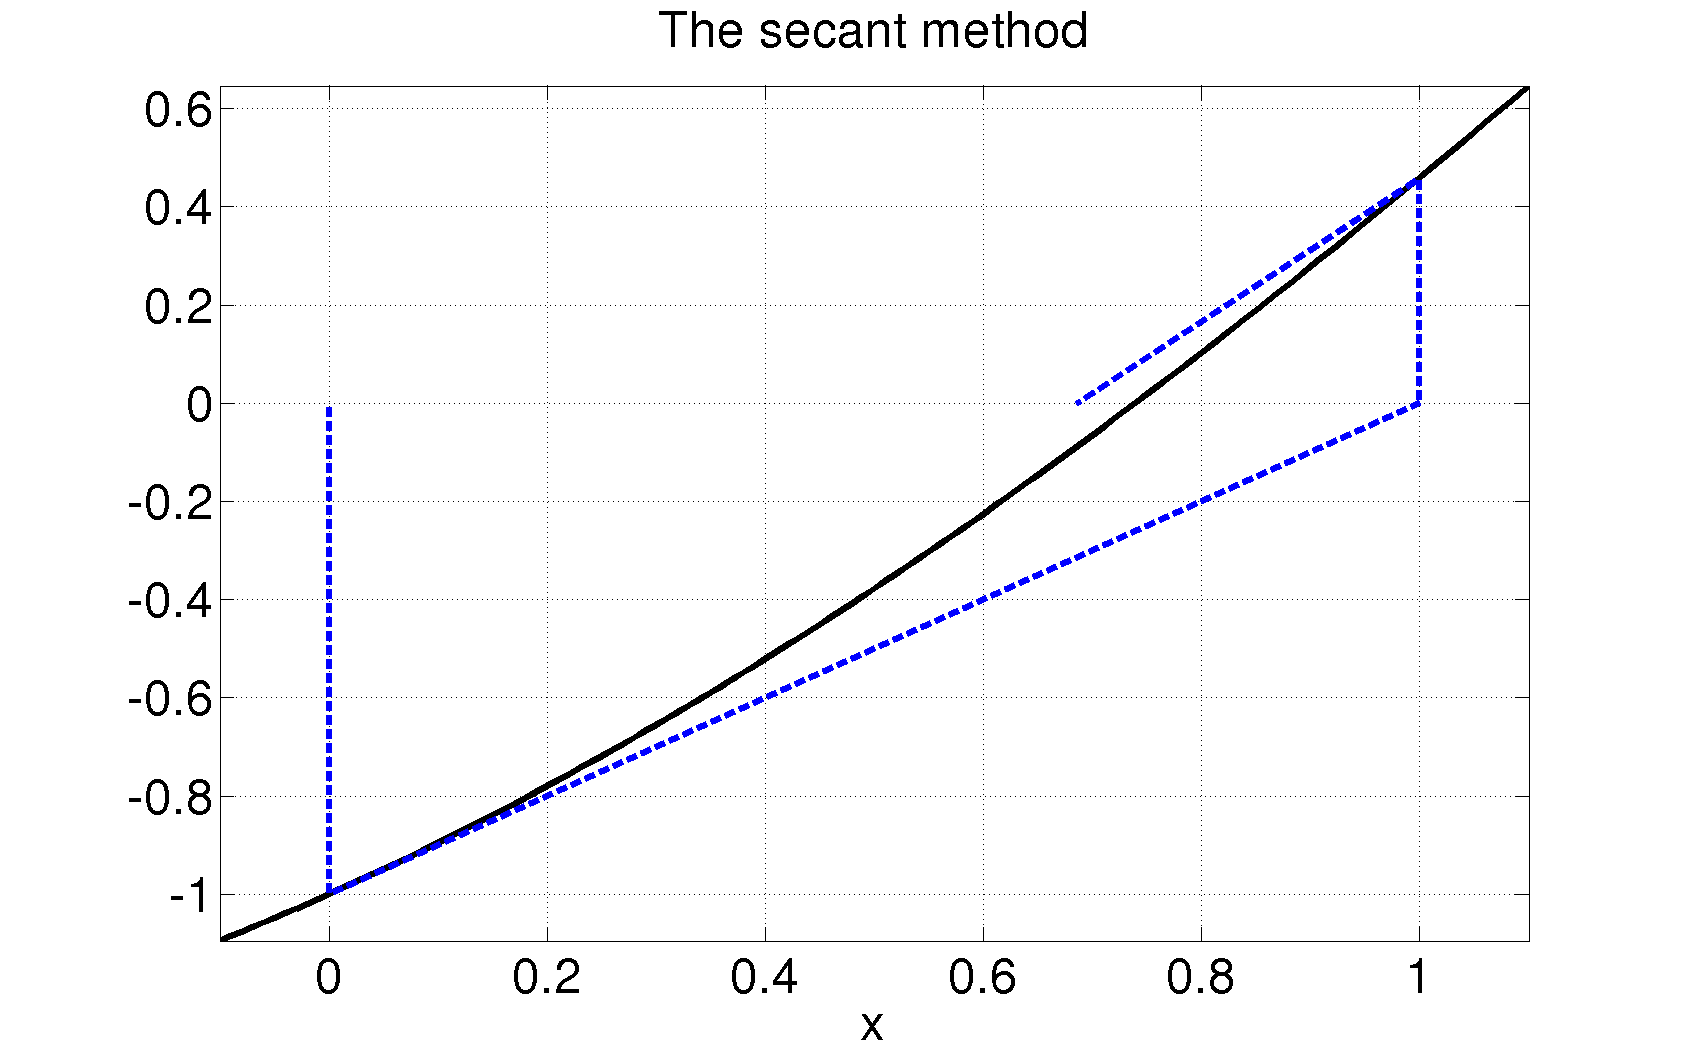
\includegraphics[width=\textwidth]{figures/SecantMap3}
          \end{center}
        }
        \only<2|handout:1>
        {
          \begin{center}
            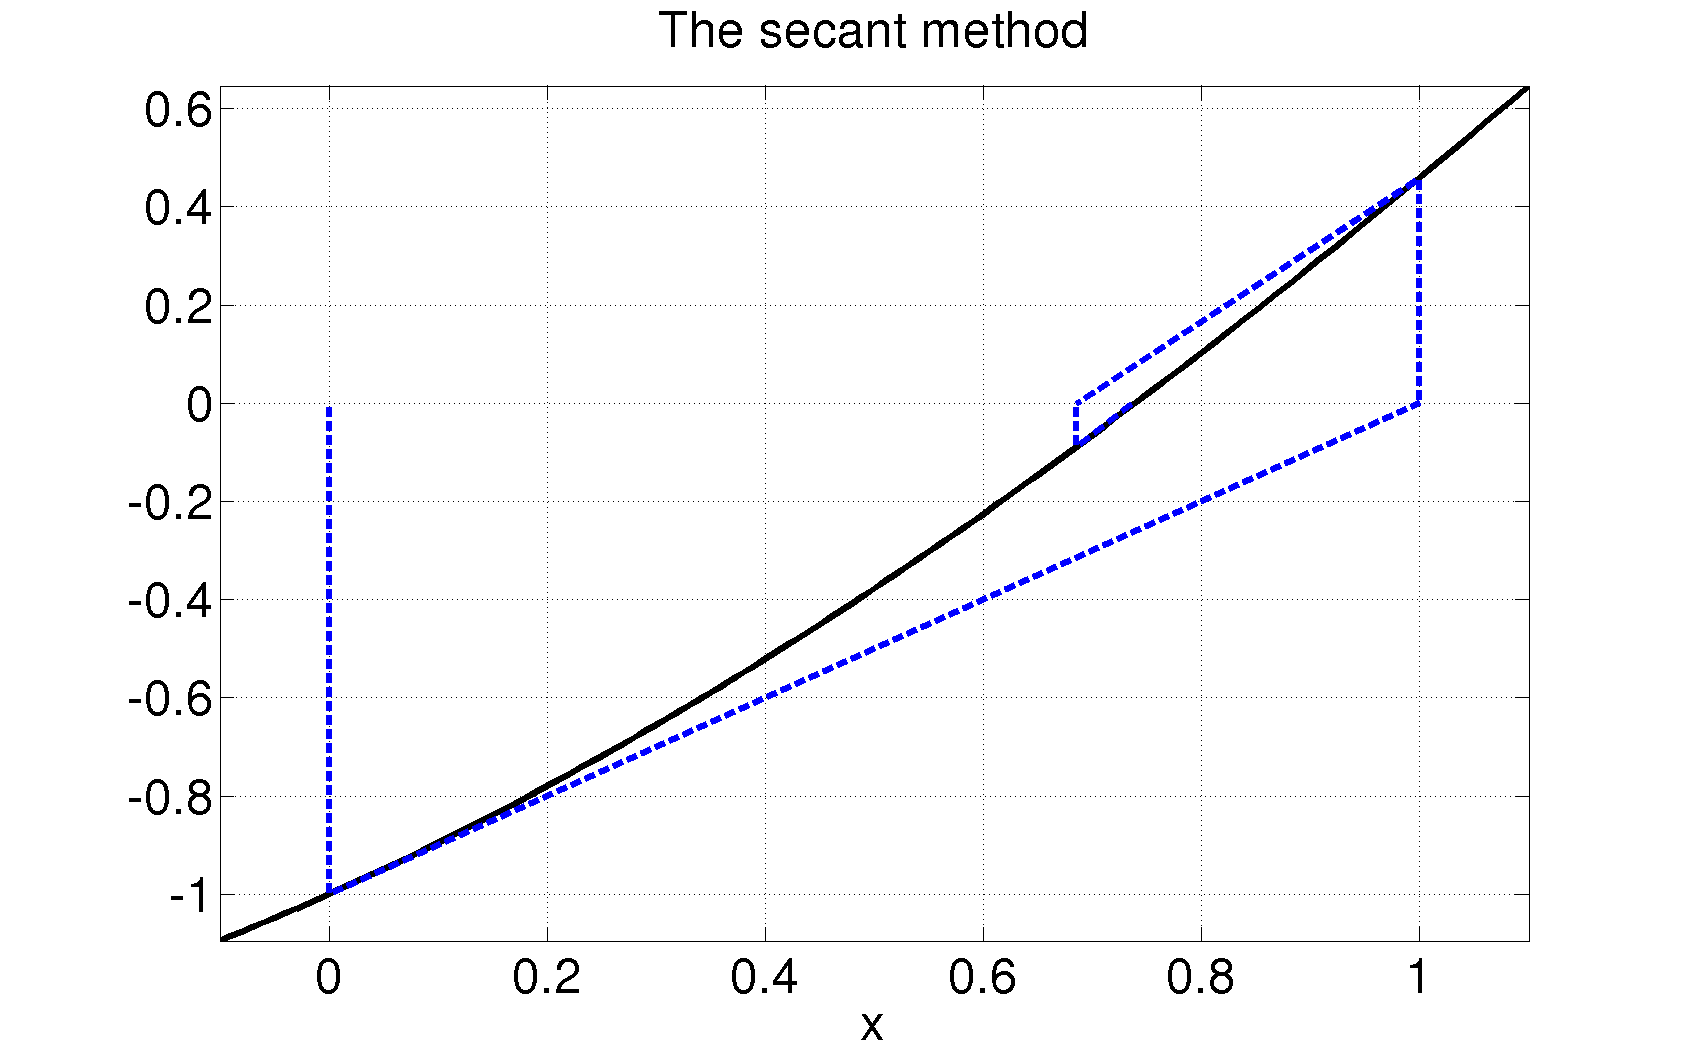
\includegraphics[width=\textwidth]{figures/SecantMap4}
          \end{center}
        }
        \only<3|handout:2>
        {
          \begin{center}
            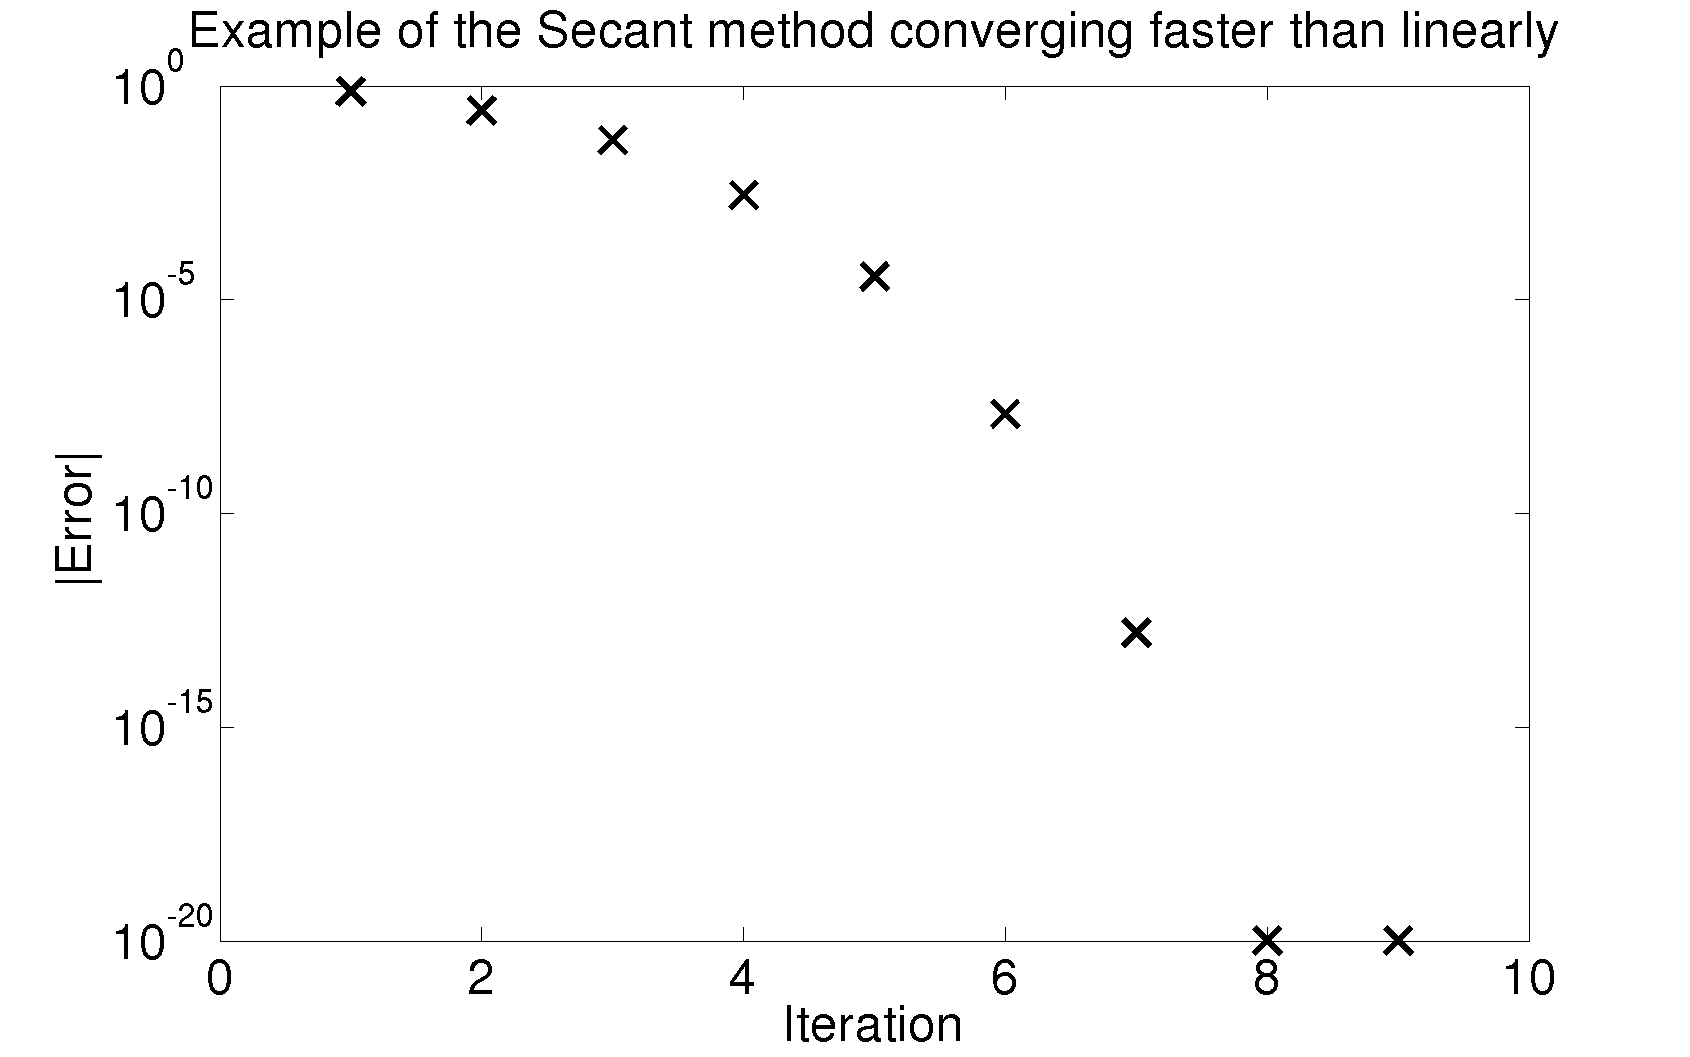
\includegraphics[width=\textwidth]{figures/Secant1}
          \end{center}
        }
      \end{overlayarea}
    \end{column}
  \end{columns}
\end{frame}


\section{Summary}


\subsection{Summary}

\begin{frame}
  \frametitle{Summary}

  \begin{itemize}
  \item The speed of convergence from the error bound using the
    Lipschitz constant $L$ is the worst-case scenario. Normally we
    expect the speed of convergence to be determined by properties of
    the map near the root $s$.
  \item By generalizing our iterative map to
    \begin{equation*}
      g(x) = x - \varphi(x) f(x), \quad \varphi(x) \neq 0
    \end{equation*}
    we still have that fixed points of $g$ are roots of $f$, but can
    speed convergence by varying $\varphi$.
  \item The more derivatives of $g$ that vanish at the root, the
    faster the convergence, but the better the initial guess must be.
  \item The chord method and Newton's method fit in this general
    framework and converge linearly and quadratically respectively.
  \item The secant method does not fit in this framework. It takes
    more iterations to converge than Newton's method, but is often
    faster in practice.
  \end{itemize}

\end{frame}

\end{document}



%%% Local Variables:
%%% mode: latex
%%% TeX-master: t
%%% End:
